%------------------------------------------------------------------------------
\chapter{Results}
\label{ch:results}

Images everywhere and proper analysis of what the user is seeing, what is failing and why.
Include default Maya fire effect, pictures of fire from the papers mentioned in the previous work section and a historical overview on the improvements in the shaders.

In order to provide a wider comparison that is not only limited to academic results, we will also confront our results with work from industry software.
FumeFX~\cite{FumeFX} is a popular tool for modelling volumetric effects, it has been used in several films and video games, e.g. Ghost Rider 2, Thor, Green Lantern, Warhammer Online and Tomb Raider: Underworld.
A frame from a fire scene in Ghost Rider 2 is shown in Figure~\ref{fig:fumefx}.
Since \Maya was used as the base platform for the development of our software, an interesting comparison should include \Mayash's fire effect.
A simple scene with plane, a sphere, a cylinder and a light was created, as shown in Figure~\ref{fig:maya_no_fire_mental_ray}.
The result of rendering the scene with \Mayash's software renderer is shown in Figure~\ref{fig:maya_fire}, note how the sphere and cylinder do not experience any change in their illumination with respect to the scene without the fire.
If \MentalRay is used to render the same scene, the image shown in Figure~\ref{fig:maya_fire_mental_ray} is generated.
Although the fire itself looks more realistic, the only alteration in neighbouring objects  is the appearance of erroneous shadows.

\begin{figure}[htbp!]
	\centering
	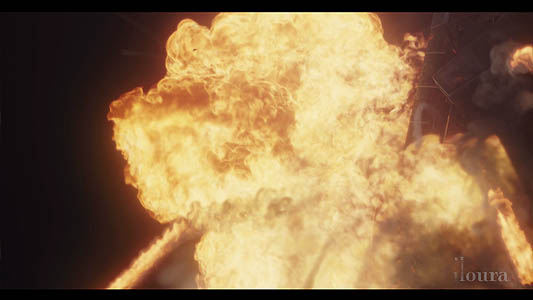
\includegraphics[width=\textwidth]{img/fumefx}
	\caption{Fire created with FumeFX~\cite{FumeFX}.}
	\label{fig:fumefx}
\end{figure}

\begin{figure}[htpb!]
        \centering
        \begin{subfigure}[t]{\textwidth}
                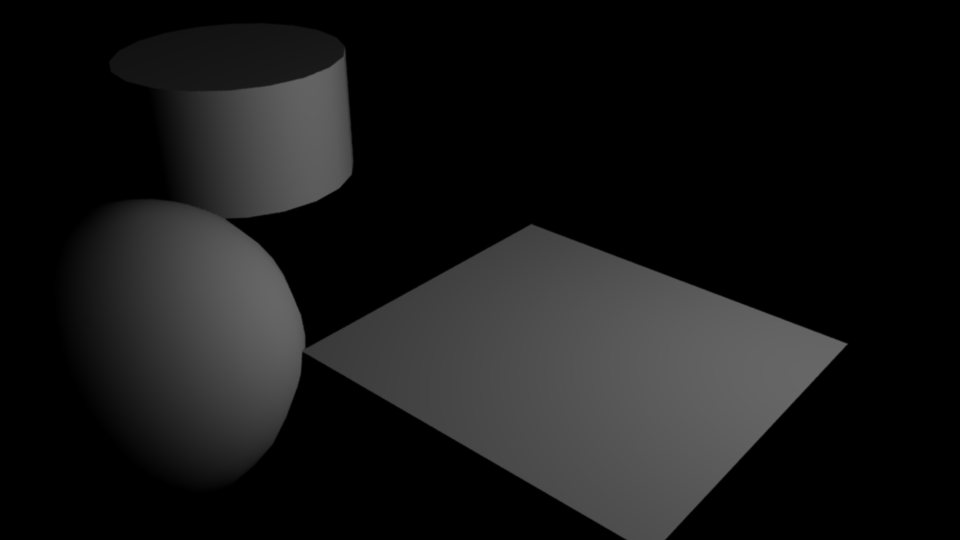
\includegraphics[width=\textwidth]{img/maya_no_fire_mental_ray}
                \caption{Scene without fire in \Maya, rendered with \MentalRay.}
                 \label{fig:maya_no_fire_mental_ray}
        \end{subfigure}    
        \\     
\end{figure}

\begin{figure}[htpb!]
		\ContinuedFloat
		\begin{subfigure}[t]{\textwidth}
                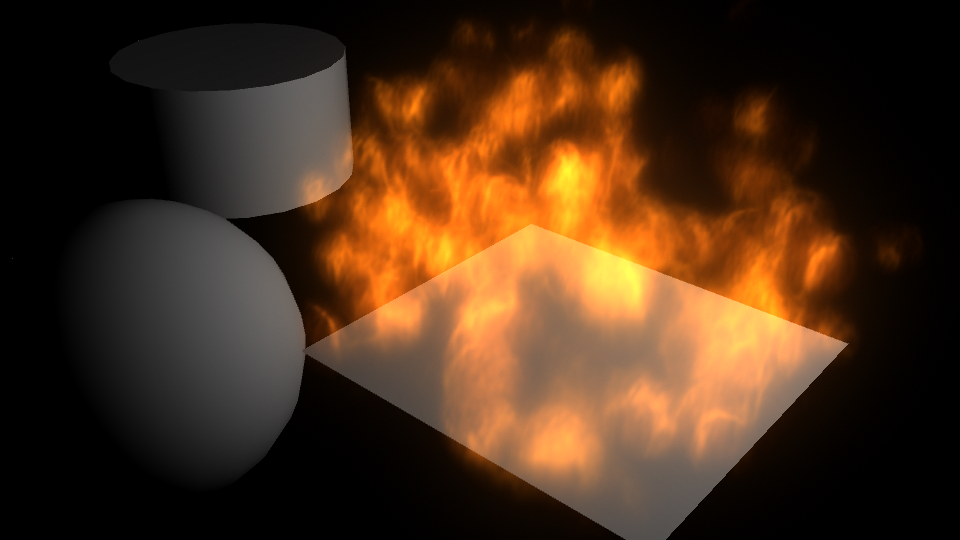
\includegraphics[width=\textwidth]{img/maya_fire}
                \caption{\Maya fire effect on a plane, rendered with \Maya software.}
                \label{fig:maya_fire}
        \end{subfigure}%        
\end{figure}

\begin{figure}[htpb!]
        \ContinuedFloat
 		\begin{subfigure}[t]{\textwidth}
                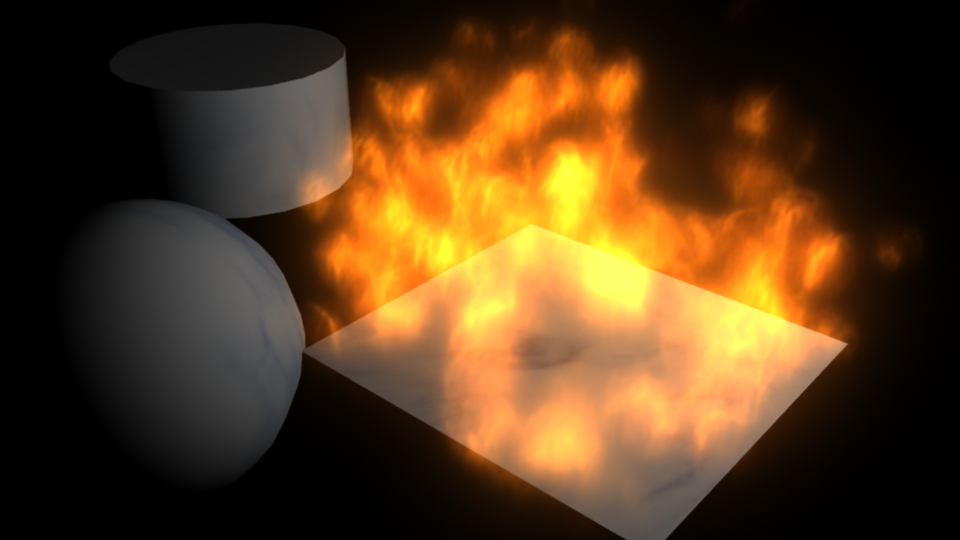
\includegraphics[width=\textwidth]{img/maya_fire_mental_ray}
                \caption{\Maya fire effect on a plane, rendered with \MentalRay.}
                \label{fig:maya_fire_mental_ray}
        \end{subfigure}%             
        \caption{Render tests for \Maya default fire effect.}
        \label{fig:maya_fire_scenes}
\end{figure}

\begin{figure}[htbp!]
	\centering
	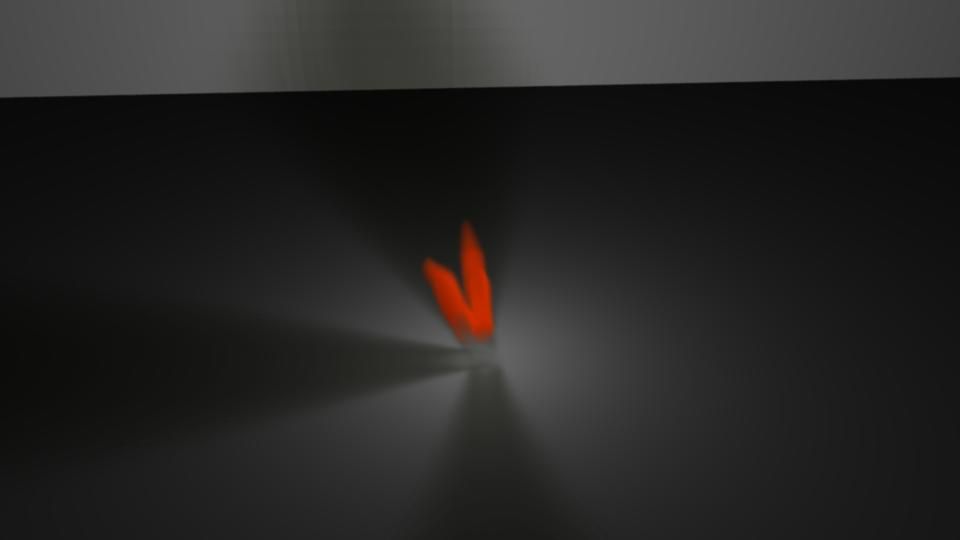
\includegraphics[width=\textwidth]{img/result_early_stage}
	\caption{Our renderer, early test, basic ray marching.}
	\label{fig:result_early_stage}
\end{figure}

\begin{figure}[htbp!]
	\centering
	
\includegraphics[width=0.25\textwidth]{img/result_synthetic}
	\caption{Our renderer, early test, basic ray marching.}
	\label{fig:result_synthetic}
\end{figure}

\begin{figure}[htbp!]
	\centering
	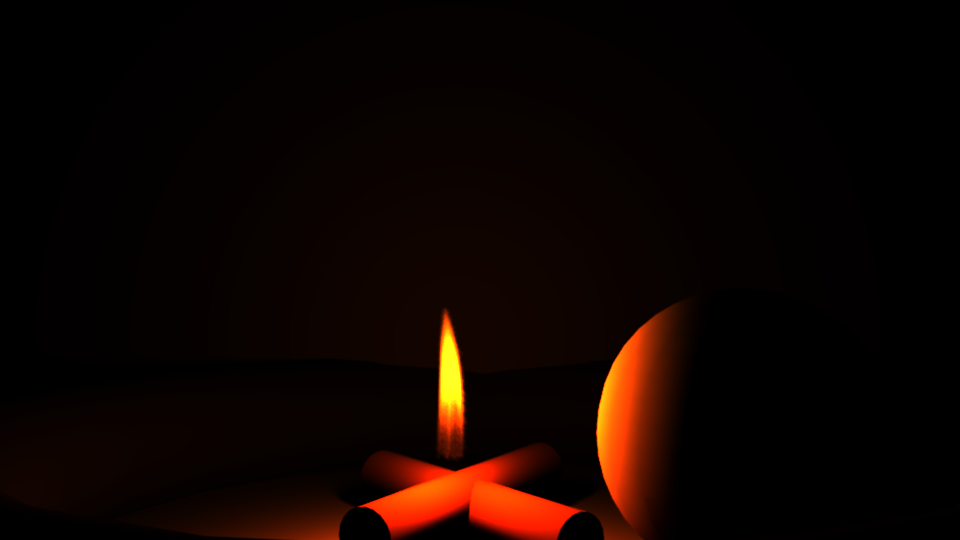
\includegraphics[width=0.8\textwidth, trim={8cm 0 8cm 10cm}, clip]{img/result_blackbody}
	\caption{result blackbody.}
	\label{fig:result_blackbody}
\end{figure}

\begin{figure}[htbp!]
	\centering
	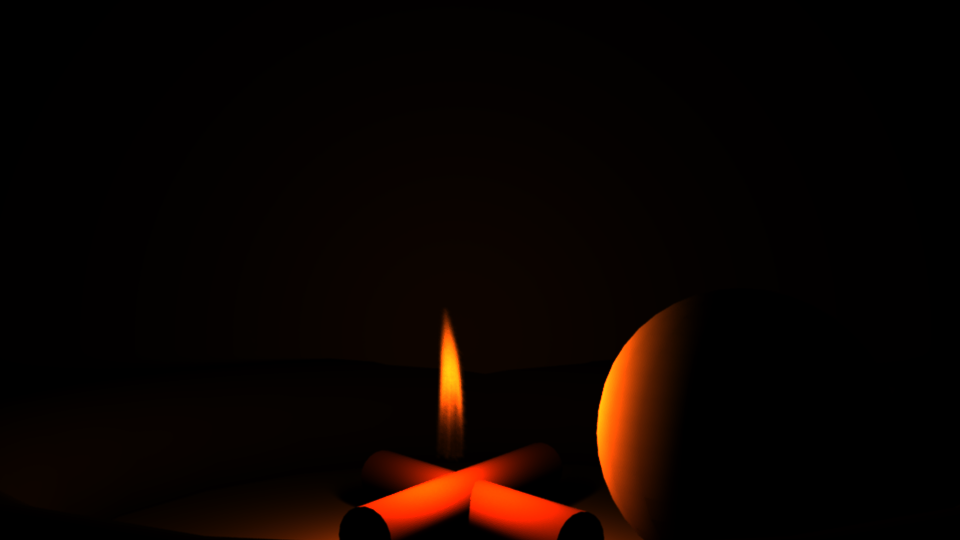
\includegraphics[width=0.8\textwidth, trim={8cm 0 8cm 10cm}, clip]{img/result_propane}
	\caption{result propane.}
	\label{fig:result_propane}
\end{figure}

\begin{figure}[htbp!]
	\centering
	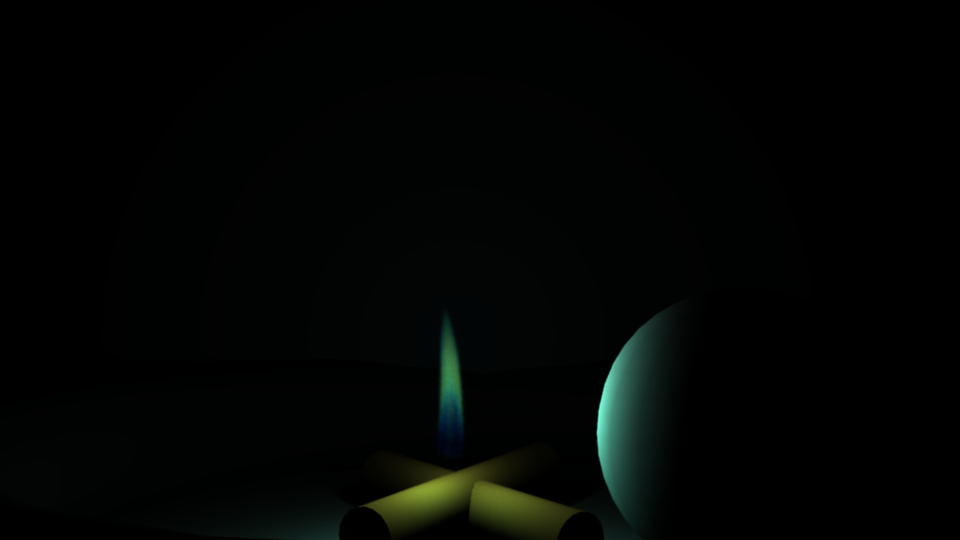
\includegraphics[width=0.8\textwidth, trim={8cm 0 8cm 10cm}, clip]{img/result_copper}
	\caption{result copper.}
	\label{fig:result_copper}
\end{figure}

\begin{figure}[htbp!]
	\centering
	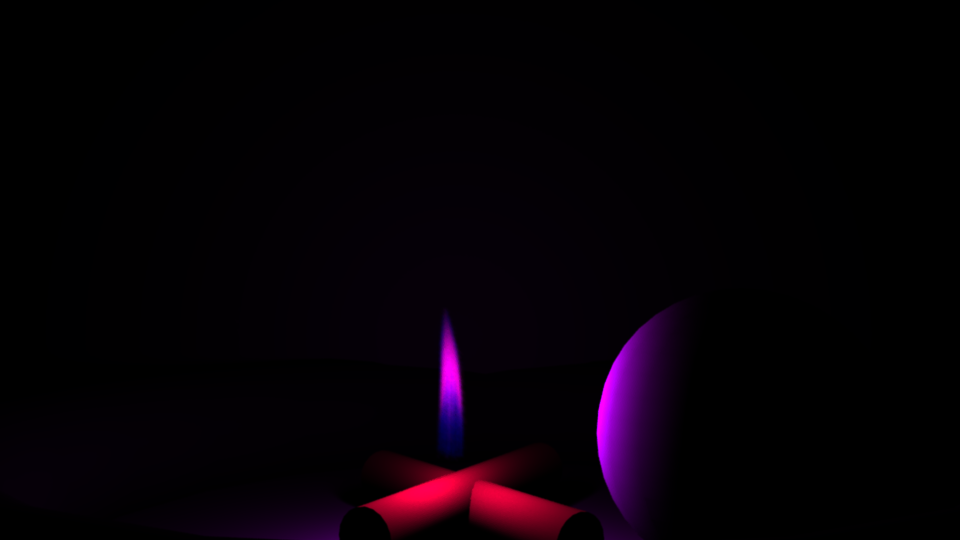
\includegraphics[width=0.8\textwidth, trim={8cm 0 8cm 10cm}, clip]{img/result_sulfur}
	\caption{result sulfur.}
	\label{fig:result_sulfur}
\end{figure}